\begin{tcolorbox}
\chapter{2009 --- Brezzvezdna Noč}

The 2009 Brezzvezdna Noč expedition was extremely successful, with 4
weeks spent in the field camping by special permission in the Triglav
national park on Tolminski Migovec. A slideshow presentation was given
at the end of the expedition in the Tolmin library by Andrej Fratnik
(JSPDT) and Jarvist Frost (ICCC), translated to Slovene by Jana Carga
(JSPDT/ICCC). Our findings were also presented as a lecture at the BCRA
2009 conference by Jarvist Frost.

In the \emph{Vrtnarija} system (5.70 km/802 m at beginning of expo) we
installed a camp at --254 m in an until now torturous parallel shaft
series (\emph{Captain Kangaroo}). This was the major factor that enabled
us to add 225 m of depth to the \emph{Dark Tranquillity} series,
connecting two wings of \emph{Vrtnarija} and creating a stunning 562 m
deep alpine exchange trip. In addition we performed three major climbs
in the area of the camp in an attempt to connect \emph{Vrtnarija} to
Sistem Migovec (11.52 km, 970 m deep), pushed \emph{Tolminska Korita}
(below the main pitch series in \emph{Vrtnarija} at -550 m) a further
--45 m, and pushed upstream above the \emph{Red Cow} sump at -750 m to
discover an aven fed watershed and an active pitch series. We now have
five major leads all at a depth greater than 500 m.

In the \emph{M2} part of Sistem Migovec, progress was slower but an
aided climb was made to a phreatic series that terminates in a drafting
boulder pile, and now forms the closest approach between the two
systems.

In all, we discovered 854 m of new passage in \emph{Vrtnarija} (bringing
the total polygon length to 6.58 km) and 101 m in smaller caves and digs
on the surface, bringing the total for Migovec to 22.9 km. An updated
survey of \emph{Vrtnarija} (in extended elevation) has been prepared,
including transformation of all mountain survey data into grid north.

\end{tcolorbox}
\backgroundsetup{
    scale=1,
    color=black,
    opacity=1,
    angle=0,
    contents={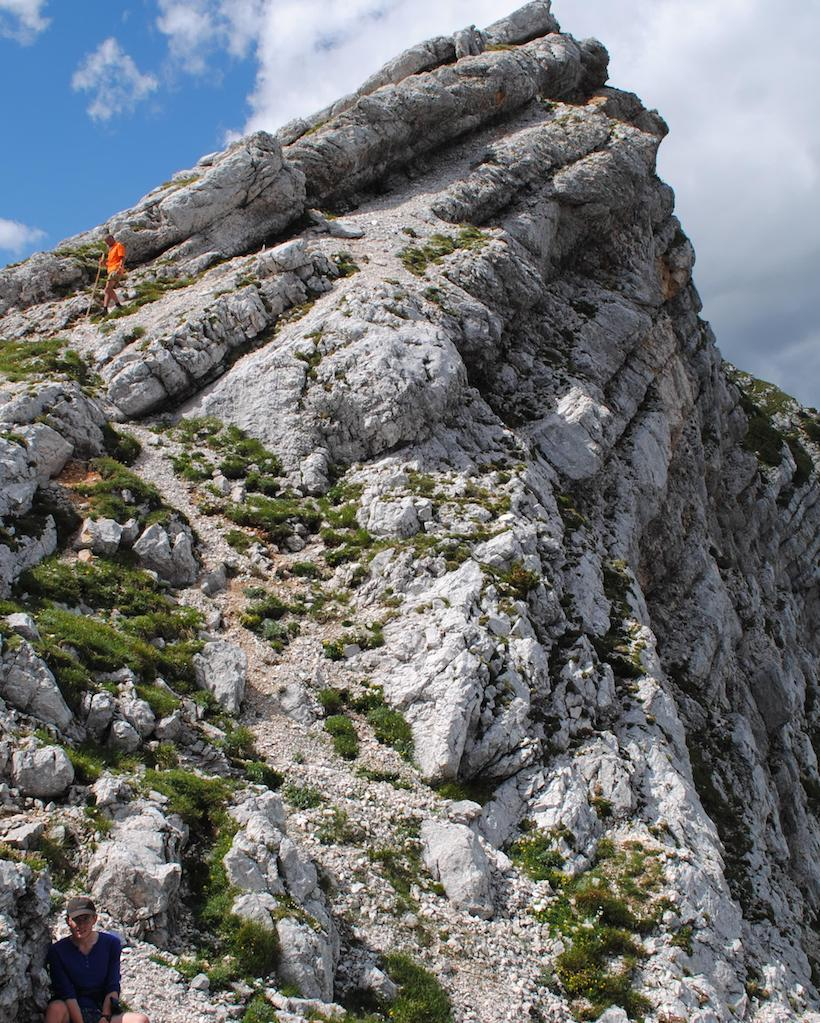
\includegraphics[height=\paperheight]{2007/intro/kuk-2013.jpg}}
}
\BgThispage









